\section{開発成果の特徴}
%開発成果のアピールポイント・特徴をわかり易く簡潔にまとめてください。
%既存の技術や製品と比較することが可能であれば、既存の技術・製品と開発成果とを対比させて記述してください。
\subsection{開発成果のアピールポイント}
本プロジェクトでは,主観的な経験を通じて視覚の多様性を理解するデバイスを開発した.
プロジェクトの特徴としては,従来の音響化 (sonification) 研究が目指している視覚障害者を主な対象とした障害者支援の文脈ではなく,「あらゆる人を対象として異なる知覚様式を体験してもらうこと」を目指した点にある.我々は多くの展示の機会を通じて「視覚には多様性がある」という思想を多くの人に広めてきた.
本デバイスの特徴は,アフォーダンスを音に変換するというかつてない「視覚的情報→聴覚的情報」変換手法をソフトウェアによって実装した点にある.また,多くの人に一目見ただけで「視覚には目は必要ない」というコンセプトを伝え,かつ現実的な使用に耐えられるハードウェアのデザインを開発したことにある.

\subsection{展示}
本プロジェクトのアピールポイントとして,多くの展示の機会を通じて「視覚には多様性がある」という思想を多くの人に広めてきたということを述べた.ここでは,Sightプロジェクトの行った広報活動である展示や記事掲載などを元に,Sightが社会に与えたインパクトについて記す.


本プロジェクトでは,「Sightを通して得られる体験は実際に足を運んで装着してみないと伝わらない」ということを早期のプロトタイピングから認識していた.そのため,本プロジェクトの目標を達成するため,我々は開発期間を通じて目標とした性能を発揮できるプロダクトを制作するだけではなく,より多くの人に知ってもらい,体験してもらう取り組みを用意してきた.

本プロジェクトでは,開発期間を通して,東京大学制作展、デジタルコンテンツエキスポ、東京藝術大学「障がいとアーツ」プログラムなど、様々な形でSightを展示し,システムの改良を重ねながら累計500名以上の方々に各バージョンのSightを試していただいた.
下記に主な展示を行ったイベントの一覧を示す.

\begin{itemize}
 \item 東京大学制作展EXTRA 2015年7月10日-7月13日
 \item デジタルコンテンツEXPO2015 2015年9月
 \item 東京大学制作展 2015年11月20日-7月23日
 \item 東京藝術大学COI「障がいとアーツ」イベント 2015年12月5日-12月6日
\end{itemize}


\begin{figure}[h]

\begin{minipage}{0.49\columnwidth}
\begin{center}
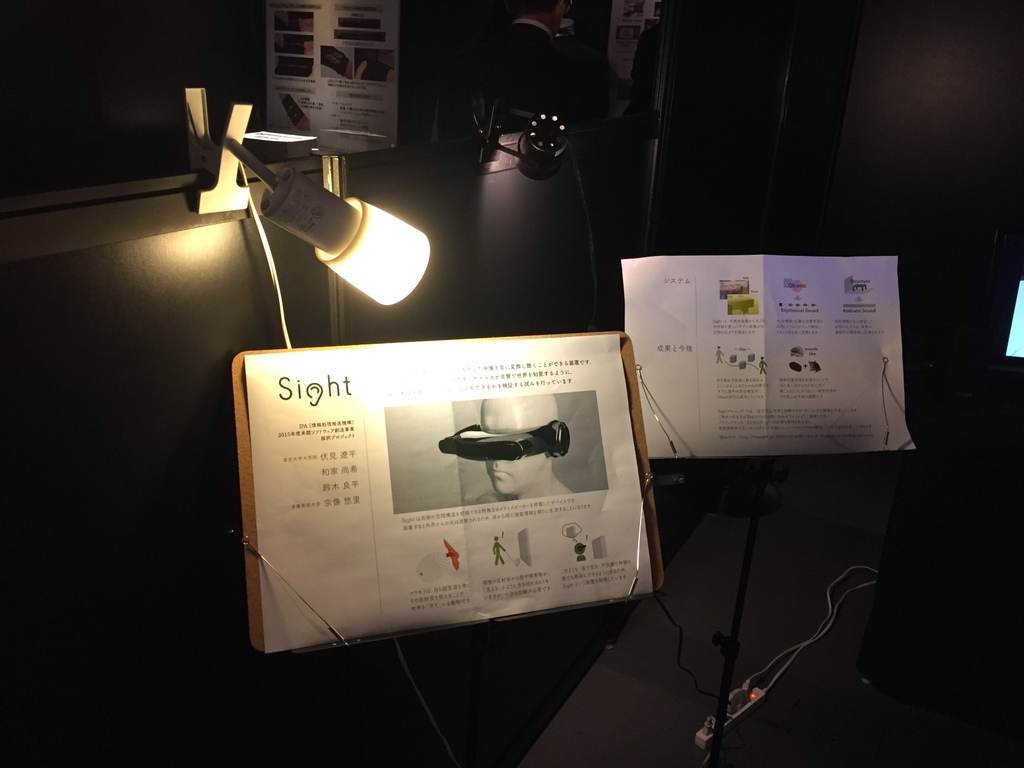
\includegraphics[height=40mm, bb=0 0 1024 768]{images/publicity/DCEXPO1.jpg}
\caption{デジタルコンテンツEXPOでの展示}
\end{center}
\end{minipage}
\begin{minipage}{0.49\columnwidth}
\begin{center}
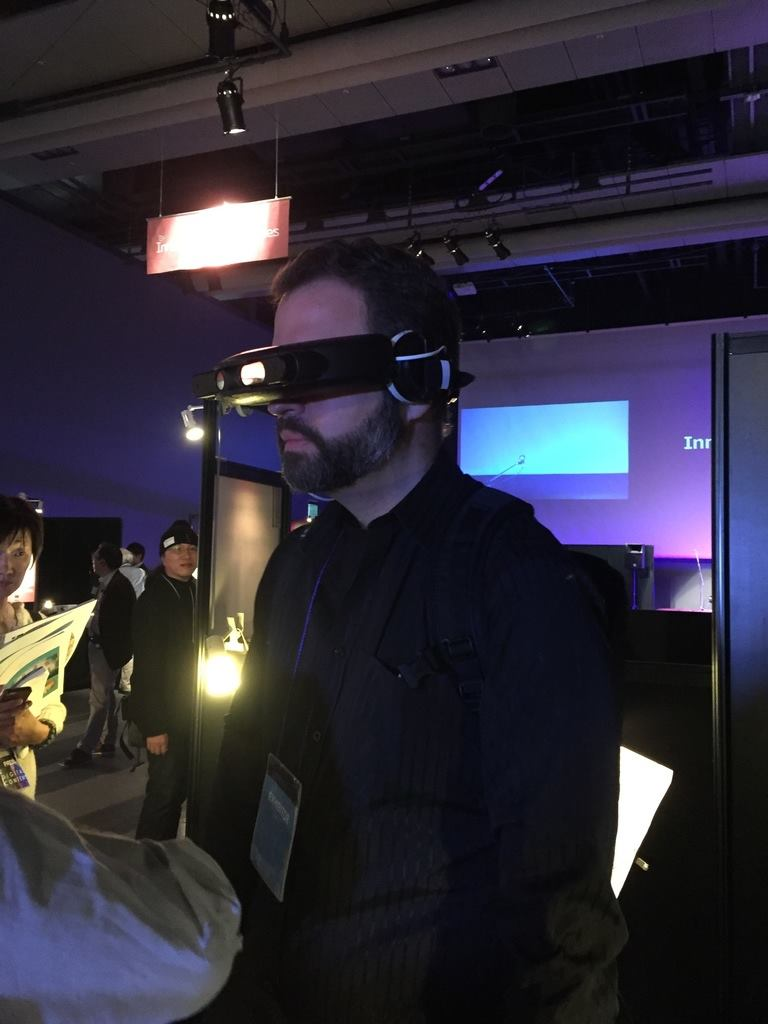
\includegraphics[height=60mm, bb=0 0 768 1024]{images/publicity/DCEXPO2.jpg}
\caption{体験者の様子}
\end{center}
\end{minipage}

\end{figure}


これらの展示来場者の方々はごく短い時間の体験が大部分だったので,長時間の装着を通じたSightならではの感覚体験を報告が得られたのはごく一部であった.
また比較的長時間試していただいた方にも上達速度にはばらつきがあり,
数分間で壁の配置などを把握できるようなった方もいれば,もっと長時間試してもなかなか把握することができないという方もいた.

デジタルコンテンツEXPOでは,今後の開発指針の策定のためにアンケートを日本語・英語で作成・配布したところ,下記のような感想が多く集まった.

\begin{itemize}
 \item 机の壁や位置がわかった
 \item どういう仕組なのか気になった
 \item 音から周りの光景を想像することができた
 \item ドキドキした・楽しかった
\end{itemize}

結果として,未踏プロジェクト期間中に,プロジェクトについて広く知っていただくために意識して多くの展示機会を得るように努力したことは,
開発の指針,とくにエンターテインメントとしてのSightの体験をより磨いていくために非常に有益であった.
また結果として,500名以上の体験者からの感想を集めることができたこと,そのうちいくらかの体験者には,人間の知覚の可塑性についての何らかの示唆を与えることができたことは,本プロジェクトの目指すところと一致した.

\subsection{広報}
先述の展示と併せて,我々の考える「視覚には多様性がある」という思想を伝え,さらに,展示に足を運んで実際に体験してもらうために,メディアを通じた広報活動も積極的に行った.

未踏のプロジェクト期間中から,Innovative Technologies受賞で得たデジタルコンテンツEXPO展示の機会などを
広報のために最大限に利用するために,展示を体験したプレス関係者のために,未踏で使っているプレゼン資料や,
記事に使える代表的な画像をまとめたプレキットを用意し,広報関係者の方に,インターネット経由で配布を行った.
結果として,下記の媒体に露出を得ることができた.

\begin{itemize}
 \item withnews 2015年1月1日『「ハッカソンはビジコンじゃない」 東大の硬派なコンペに強者続々』
 \item gizmodo 2015年7月13日 『人間はどこまで進化できるのか? "音で見る"感覚拡張デバイス「Sight」開発者インタビュー』
 \item 攻殻機動隊REALIZE project 2015年7月27日 『2029年の義体を一部体感。「東京大学制作展エクストラ2015 グッバイ・マイ・ボディ」展参加。視覚や聴覚・感情をハックする作品で攻殻機動隊世界を検証』
 \item IGNITION 2016年1月 『New VR Headset Invites Users to “See with Their Ears”』
\end{itemize}

\begin{figure}[h]
\begin{center}
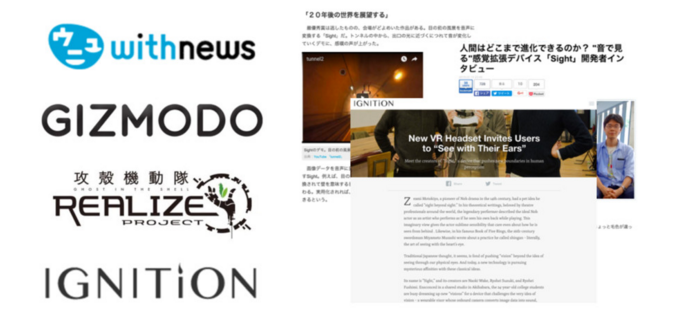
\includegraphics[width=120mm, bb=0 0 674 330]{images/publicity/publicity.png}
\caption{掲載いただいた主なメディアと記事内容}
\end{center}
\end{figure}


これらの記事を見た一般の方や広報関係者が最終成果発表のプレゼンテーションやデモに足を運んでくださり,
次のメディア取材などにつなげることができており,プロジェクト期間を通して非常によいサイクルを形作ることができた.

また,プロジェクトメンバーは全員,広報活動に関する経験がなかったため,このようなパブリシティサイクルの形成に携われたことは非常に価値ある経験となった.








